% *******************************************************************************
% * Copyright (c) 2007 by Elexis
% * All rights reserved. This document and the accompanying materials
% * are made available under the terms of the Eclipse Public License v1.0
% * which accompanies this distribution, and is available at
% * http://www.eclipse.org/legal/epl-v10.html
% *
% *  $Id: notizen.tex 2467 2007-06-02 16:36:36Z rgw_ch $
% *******************************************************************************
% !Mode:: "TeX:UTF-8" (encoding info for WinEdt)

\section{Notation dans Elexis}
Ce Plugin permet d'administrer des documents et notes qui ne se réfèrent pas à un patient spécifique mais qui sont plutôt d'intérêt général ( pense-bêtes, Guidelines, Trucs et astuces, modèles etc). Veuillez ouvrir la perspective dans laquelle vous souhaitez intégrer votre \textit{bloc-notes}et choisissez \textit{fenêtre - affichage - autres}. Sélectionnez là la View \textit{bloc-notes}.

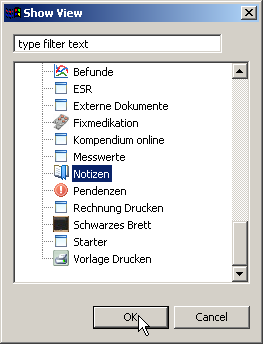
\includegraphics[width=3in]{images/notizen1}
% notizen1.png: 263x344 pixel, 96dpi, 6.96x9.10 cm, bb=0 0 197 258

La fenêtre suivante s'ouvre (mais chez vous probablement encore sans contenu):

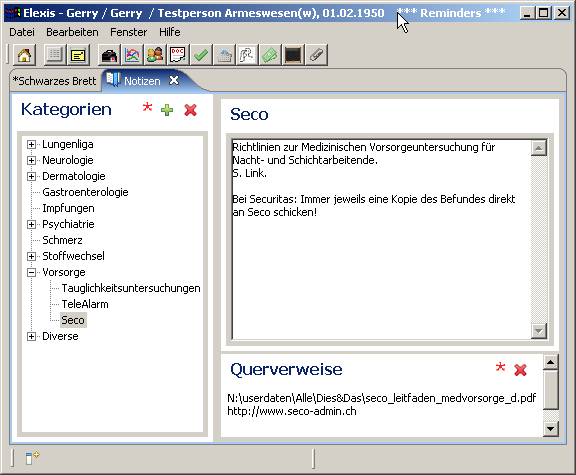
\includegraphics[width=3in]{images/notizen2}
% notizen2.png: 576x475 pixel, 96dpi, 15.24x12.57 cm, bb=0 0 432 356

Les notes peuvent être structurées de façon libre et classées de façon hiérarchique. Toute note peut contenir du texte, des références vers un document externe ou des sous-catégories.

\begin{itemize}
 \item Pour créer une nouvelle catégorie principale veuillez cliquer sur le symbole de l'étoile sous \textit{Catégories}.
\item Pour cérer une nouvelle sous-catégorie d'une note, veuillez marquer la note et cliquez ensuite sur le sympbole Plus sous \textit{Catégories}.
\item Pour effacer une note  y inclus toutes ses sous-catégories veuillez cliquer sur le Symbole X sous \textit{Catégories}.
\item Pour introduire un texte pour une catégorie ou une note veuillez le taper dans la fenêtre à droite. Il sera sauvegardé automatiquement  et vous pouvez le changer à tout moment.
\item Pour attribuer un fichier externe ou un site internet à une note ou une catégorie veuillez cliquer sur le symbole d'étoile sous \textit{références}. Vous pouvez y introduire le chemin d'accès à ce fichier respectivement l'adresse URL pour le site internet.
\item Pour voir ou adapter un fichier relié veuillez double-cliquer sur la référence.
\item Pour effacer une référence (mais pas le fichier lui-même !) veuillez cliquer sur le symbole X sous  \textit{références}.
\end{itemize}

\subsection{notes explicatives}

\begin{itemize}
 \item Les notes sont sauvegardées dans la base de données est sont accessibles par principe depuis tous les postes de travail connectés et par conséquent elle peuvent être vues par tous les utilisateurs.
\item Les fichiers reliés ne sont que reliés et ne sont pas importés dans la base de données. L'accès à ces fichiers ne fonctionne depuis d'autres postes de travail que lorsque dans ces postes le même chemin a été relié à ces fichiers - en général ceci est le cas lorsqu'il s'agit d'un répertoire commun sur le serveur.
\item L'ouverture des fichiers reliés se fait par l'application prévue dans le système d'exploitation. Par exemple Acrobat Reader pour des fichiers PDF. Pour cette raison on pourra naturellement ouvrir ces fichiers que sur les postes de travail où l'application spécifique est installée.

Pour intégrer cette fenêtre de façon durable dans la perspective choisie veuillez suivre \textit{fenêtre-sauvegarder la perspective}.

